We propose a mathematical model of a WA based on an extension of the simple graph generally adopted to model pages and links between pages. The verification procedure consists of six principal steps: 
\footnotesize
\begin{enumerate}
	\item Modeling of the system as finite state machine;
	\item Manual verification of some route in the graph to immediately check problematic state transitions in the model (optional);
	\item Formalization of fundamental correctness properties as \ctl axioms to be verified in the model;
	\item Automatic verification by means of model checker to verify accuracy of \ctl axioms in every state;
	\item Analysis of possible explanations provided by model checker (only if a violation of a specification occurs);
	\item Correction and refinement of the WA design.
\end{enumerate}

\normalsize
In the following subsections, we describe each step.



\subsection{Modeling a Web Application}
Most intuitive and immediate model of a WA can be built by means of logical associations from state to state, where each of them represents a web page whereas transitions represent links connecting web pages \cite{de-alfaro-01}. This kind of representation is very simple, but theoretically it is more correct also consider links as states of the model, because in this way a verification of properties related to coherence and consistence of connections can be performed.

In general, due to complexity of the hypertextual structure of the Web, a WA cannot be modeled using a simple graph structure where nodes represent pages and arcs represent hyperlinks. In fact, the widespread use of frames, while controversial, makes a window be composed by several pages. To solve this question, in previous paper we proposed \cite{seke-02} \cite{csmr-03}, we identified a new kind of object in a WA and consequently a new kind of state in the model, that is the ``window'' state. A generic window could be divided in one or more frames where one or more web pages can be loaded.

Last essential question in WA modeling is to distinguish between links connecting to other web pages and links triggering an action of the server (for example, the download of a file or login operations). Hence, we extend the WA model to include ``action'' states representing actions performed in a specific web page, typically said ``Server Page''. In the paper \cite{disc-doni-mong-tota-cast}, WAs are modeled as FSM where pages, links, windows and actions are states. 

In what follows we resume and formalize above considerations by means of two definitions.

\footnotesize
\begin{definition}\label{def:graph}
A Web Application Graph (WAG) is a graph $G=(N,C)$ where nodes $N$ are divided as
$N=W \cup P \cup L \cup A$ (Windows, Pages, Links and Actions), such that:
\begin{enumerate}
   \item $W, P, L, A$ are pairwise disjoint, \ie $W \cap P= \emptyset$, $W
   \cap L= \emptyset$ $W \cap A = \emptyset$ $L \cap P = \emptyset$ 
   $L \cap A = \emptyset$ $P \cap A = \emptyset$ and

   \item arcs connect only windows with pages, pages with links or actions, 
   links with windows and actions with windows, \ie $C \subseteq (W \times P) 
   \cup (P  \times (L \cup A)) \cup((L \cup A) \times W)$;

	 \item$\forall w \in W \exists p \in P : (w,p) \in C$, that is: ``Every
	 window contains at least one page'';
 
 	 \item $\forall x \in (L \cup A) \exists w \in W : (x,w) \in C$, that is: ``Every link points
   to a window and every action creates a window''.
\end{enumerate}
\end{definition}

\normalsize

Figure \ref{fig1} depicts a simple WAG we use as reference throughout the paper.

\begin{figure}[ht]
\centerline{\scalebox{.4}{\includegraphics{figura1.eps}}}
\caption{The WAG used as example \label{fig1}}
\end{figure}

\footnotesize
\begin{definition}\label{def:path}
 A navigation path is a sequence $ w_1 w_2 \ldots w_n $ where 
 $\forall 1 < i < n-1 $
 \[
  \exists p \in P \exists x \in (L\cup A) : w_i
 \rightarrow p \wedge p \rightarrow x \wedge x \rightarrow w_{i+1}
 \]
\end{definition}

\normalsize
To express in a \ctl formalism and verify properties of the above Web Application Graph, we reserve four propositional letters $w, p, l, a$ to distinguish nodes modeling windows, pages, links and actions respectively. Hence we enforce transitions only as established in the previous Definition~\ref{def:graph}. 

Such conditions could also be verified in the WAG by checking the following \ctl formulas:

\footnotesize
\begin{itemize}
	\item $ AG(( w \vee p \vee l \vee a) \wedge(\neg w \vee \neg p) \wedge (\neg w \vee \neg l) \wedge ( \neg w \vee \neg a) 			 
						\wedge(\neg p \vee \neg a) \wedge (\neg p \vee \neg l)\wedge (\neg p \vee \neg a)\wedge (\neg l \vee \neg a))$ \\
	\item $AG (w \Rightarrow AX p \wedge p \Rightarrow AX (l \vee a) \wedge l \Rightarrow AX w \wedge a \Rightarrow AX w)$ \end{itemize}


\normalsize
\subsection{Simulation Process}
The first step of our approach is the translation of the WAG in the NuSMV formalism (model declaration language); then, a preliminary simulation could be useful for a first verification of the model behavior; it allows to check if state transitions in the SMV code are coherent with WAG.

Notice that in the specific example of WAs, the simulation process points out an important question related to Model Checking techniques, but relative to any WAG. More precisely, the declaration of state transitions forces model checker to consider specific properties for next states. The missing declaration of state transitions in any endpoint-node, \ie a node which does not allow further transitions, makes model checker free for assigning any possible value of property to non-existent next states. 

However, NuSMV does not provide any formal construct to define an endpoint-node of the graph, then we solved the problem realizing an independent endless cycle, where all the final states are connected.




\subsection{Axioms of correctness}
By means of Model Checking techniques, we test the validity of interesting properties (related to typical features of a WA) in the model. 
To formalize axioms of correctness, we use following ``labels'' to name some state in the WAG:

\footnotesize
\begin{itemize}
	\item \textbf{private} denotes that a window or a page contains private information, hence it is visible only to a specific category of users;
	\item \textbf{login, logout} denotes that in the current state the server is busy because it is performing either a user login action or a user logout action;
	\item \textbf{error} denotes that a page contains an error message.
\end{itemize}

\normalsize
First of all we must check the correct use of propositional letters $w, p, l, a$ in the model by imposing the following \ctl specification:

\footnotesize
\begin {itemize}
	\item $private$ is applicable only to pages or windows, so it is not applicable to links or actions\\$AG(l \vee a \Rightarrow \neg private)$
	\item $ login $ and $ logout$ are applicable only to actions \\$AG(w \vee p \vee l \Rightarrow \neg login \wedge \neg logout)$ 
	\item $ error $ is applicable only to pages\\ $AG(w \vee l \vee a \Rightarrow \neg error)$
	\item a \emph{private} window must contain at least one \emph{private} page\\$AG(w \wedge private \Rightarrow EX(private))$
	\item a \emph{not private} window must not contain \emph{private} pages\\$AG(w \wedge \neg private \Rightarrow AX(\neg private))$ 
\end{itemize}

\normalsize
Furthermore, using these propositions we can check some interesting properties of a web application design. For example we can check whether the access to private page occurs through a login, hence whether it is correct:

\footnotesize
\begin{itemize}
	\item we must find some \emph{private} information after a \emph{login} action: \\ 
$AG(login \Rightarrow EF(private))$

	\item after a \emph{login} action we can make a \emph{logout} action in the future or the application must manage a \emph{login error} and it must be possible to make a \emph{login} again: \\ 
$AG(login \Rightarrow AG(w \Rightarrow EX((EX logout)\vee error)\vee EF login)$

	\item after a \emph{logout} action we can load only \emph{not private} pages before a new login:\\
$AG(logout \Rightarrow A(\neg private U  login))$

	\item the homepage must verify the following property:\\
$A(\neg private U login)$
\end{itemize} 

\normalsize
Another property of web application design concerns the error management; we can check the web application behavior when an error occurs. For instance:

\footnotesize
\begin{itemize}
	\item for every \emph{not logout} action the web application must manage eventually an \emph{error} page:\\
$AG(a \wedge \neg logout \Rightarrow EXEX error)) $
	\item the user must repeat the \emph{login} action when an \emph{error} occurs:\\
$AG(error \Rightarrow A(\neg private U login))$
\end {itemize}


\normalsize



\subsection{Verification Process and Model Refinement}
With the aid of following definitions we can introduce the concept of verification of a Web Application.

\footnotesize
\begin{definition}[Verifying a Web Application]\label{def:model checking} 
Given a WAG $G$ modeling a web application, given an initial state $s$ and a property $p$, the web application \emph{verifies} $p$ iff $p$ \emph{holds for} $s$ \emph{in} $G$. 
\end{definition}

\normalsize
In Figure \ref{fig2} we added properties to the  states in Web Application Graph used as reference. 

\begin{figure}[ht]
\centerline{\scalebox{.45}{\includegraphics{figura2.eps}}}
\caption{The WAG with labeled properties \label{fig2}}
\end{figure}

To perform verification, WAG and \ctl specifications have to be expressed in NuSMV input language. After the automatic verification by means of the model checker, the analysis of possible possible explanations allows to understand incorrect WA behavior and to refine the model. Typically, after the first verification several faults are found in the model of the WA.

According to the above WAG, the first set of axioms we submit to the checker is the one related to state labels and atomic propositions: because the model checker does not provide any explanation, we can conclude that they are correctly assigned to states in the WAG.

Hence, we submit to NuSMV six axioms previously outlined concerning login and logout actions. The model checker identifies an error and provides corresponding explanation. In particular it shows a sequence that stops after login, because the ``private'' property is missing in a state of the WAG; hence, we will assign the ``private'' label to both ``Member'' window and ``NewsListP'' page. Remember that a private window must contains at least one private page.

To complete correct checking of these properties, we introduce a new state in the model to represent logout action which has to be preceded from a page. ``NewsListP'' page is logically the better candidate for this purpose, because it is always loaded in the assigned frame and then a user can logout at any moment. However, a fixed specification points out to insert a connection between ``Logout'' state and ``HomepageW'' state, to make possible to follow a path bringing a new login action.

Verification process goes on with the analysis of axioms related to the error management: every ``action'' state of the model implies a server elaboration phase; it could have either positive or negative result. In the last case, a correct WA should display to user an error page and should inhibit any further operation to not authorized users.

In the graph pictured in Figure \ref{fig3} an ``error'' page after ``Login'' one is shown; notice that ``Logout'' state has only a connection to ``HomepageW'' state because it does not need of a following ``error'' page (logout action cannot have a negative result). Then, we inhibit axioms verification ``Logout'' state in the following way: 

\centerline{$AG ((type=action \& property!=logout) \rightarrow EX(EX property=error))$}

However, the WA must permit to the user to restart server elaborations --after a login failure-- with right data of login. Hence, we insert in the WAG the new ``HomepageLink'' state, for representing the connection between ``error login'' page and ``Homepage''one.

\begin{figure}[ht]
\centerline{\scalebox{.6}{\includegraphics{figura3.eps}}}
\caption{WAG after verification process \label{fig3}}
\end{figure}





\subsection{Extension of the model}
Now, after performing the verification step, we can extend the WAG by means of introduction of WA access policies. We use the same previously applied approach. 

We briefly recall fundamental mechanisms of access policy in a generic WA. They essentially consist of:

\footnotesize
\begin{itemize}
	\item authentication: it confirms user identity; particularly in the form-based authentication, user has to provide name and password, they are verified and recognized by the server which can authorize or deny access;
	\item authorization: it is a process for granting specific resources to specific users; the definition of users ``roles'' and related resources is performed by WA administrator. S/He generally creates a user account and by means of it a user accesses to specific resources.
\end{itemize}

\normalsize
Hence, we extend the graph model assigning some resources to two categories of users:

\footnotesize
\begin{itemize}
	\item authorized users: they can view specific areas of the WA, not accessible to anonymous users;
	\item administrators: they can insert or cancel a new user, can view the list of authorized users and can access to all the resources of the WA. 
\end{itemize}

\normalsize
Therefore, if a user performs an access to the WA for the first time, before registration s/he is unknow for the system. Her/his login data has to be recognized and stored, then we also must introduce a mechanism of user registration. To add these features, the original graph related to the WA example has been extended as illustrated in the following Figure4.

\begin{figure}[ht]
\centerline{\scalebox{.7}{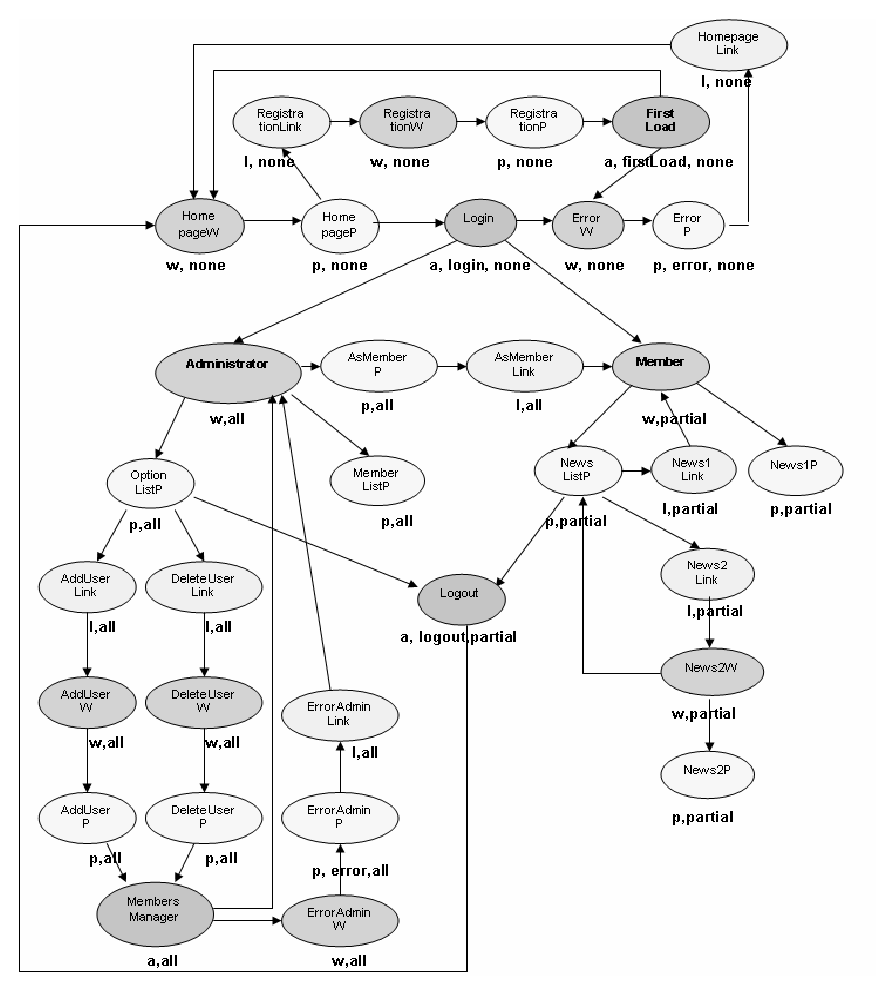
\includegraphics{figura4.eps}}}
\caption{WAG with access policies \label{fig4}}
\end{figure}

A direct consequence of such extensions is the elimination of ``private'' labels. In fact now we cannot only distinguish private pages and public pages accessible by anonymous users, but also we must distinguish private pages accessible by authorized users and private pages accessible by the administrator.

We think ``private'' label has became insufficient now, hence we introduce a new correctness axiom called ``accessibility''; it can assumes following values: 

\footnotesize
\begin{itemize}  
	\item	\textit{none} if web pages are visible by anonymous users;  
	\item	\textit{partial} if web pages are visible by authorized normal users;  
	\item	\textit{all} if web pages are visible by administrators.  
\end{itemize}

\normalsize
For the sake of simplicity, in our reference graph we consider only three users categories, but we are able to analyze models including more classes of users. They can be divided according to different levels of functionality or can be simply related to personal areas and resources (multiple subjects in the same category). Notice that possible extensions of the model does not compromise the validity of the reference example, whose correctness has been also proved in case of additional users categories.

In what follows we formalize and represent the graph grouping possible states of a user, independently by accessibility of pages s/he views at the moment. Hence we build a second supplementary model, for maintaining current states of users during navigation in WA: 

\footnotesize
\begin{itemize}  
	\item \textit{noLog} is an anonymous user which did not perform login operations;  
	\item \textit{member} is an authorized user which performed login as user of the WA;  
	\item \textit{admin} is an authorized user which performed login as administrator of the WA.  
\end{itemize}	

\normalsize
The state transitions permitted in this model can be represented by means of the simple following graph: 

\begin{figure}[ht]
\centerline{\scalebox{.35}{\includegraphics{figura5.eps}}}
\caption{User graph \label{fig5}}
\end{figure}

To verify some important specification, we synthesize following axioms:  

\footnotesize
\begin{itemize}
	\item a member cannot have administrator functions and an anonymous user cannot view pages belonging to a member:\\  
       $AG(member \Rightarrow !all );$     $AG(noLog \Rightarrow (!partial \wedge !all))$
	\item administrator can access to resources belongings to every authorized user:\\
       $AG( admin \Rightarrow (all \vee partial))$
\end{itemize}      

\normalsize
Besides, we previously introduced some \ctl specifications, that we now must correct according to new accessibility property, by removing specifications related to the ``private'' label. In particular about:

\footnotesize
\begin{itemize}
	\item initial state (Homepage):\\
			$A( none  \cup  login )$
	\item login and access to pages:\\ 
      $AG( login \Rightarrow  EF(partial \vee all) );$      $AG( logout \Rightarrow  A(none \cup  login))$
	\item error management:\\
			$AG (login \wedge EX EX error) \Rightarrow  A(none \cup  login )$
\end{itemize}

\normalsize
The above specifications point out that the accessibility logically replaces the correctness axiom related to private pages, providing a better precision in management of private resources of different users in the WA.

Now, verification process consists of establishing if state transitions in the model are coherent with accessibility of the pages. Hence, we define further NuSMV module besides \textit{MAIN} one; by means of it we synchronize user state transitions according to WA state transitions. For this purpose we use the ``stateName'' variable passed as input parameter every time the module is started. 
